\begin{figure}[!h]
	\begin{center}
		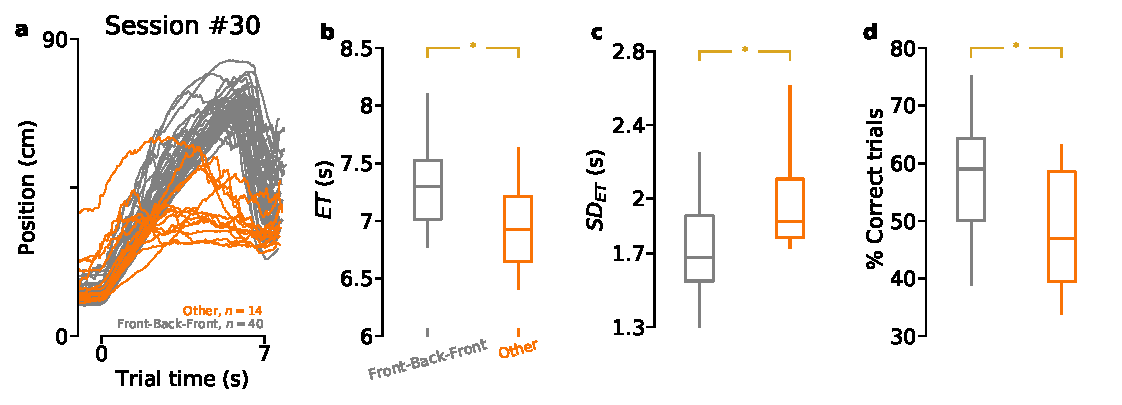
\includegraphics[width=\textwidth]{ch-appendicies/figures/BadCtrl.pdf}
		\caption[Different Control Trajectory Groups]
		{\textbf{Task proficiency according to the type of trajectory performed by animals.}
		\textbf{a)}
		Same as \Autoref{fig:time:CtrlTrd}{c, right}, but animals were divided in two groups according to whether they performed the front-back-front trajectory (gray) or not (\textit{other}, orange).
		\textbf{b)}
		Entrance times.
		$p=0.0066$ (permutation test).
		\textbf{c)}
		Standard deviation D of ET.
		$p=0.03$ (permutation test).
		\textbf{d)}
		Percentage of correct trials.
		$p=0.01$ (permutation test).
		For panels~b-d, same color code as in panel~a.
		Data from sessions~\#~$\geq20$ were averaged for each animal.
		}
		\label{fig:appendix:BadCtrl}
	\end{center}
\end{figure}